\documentclass{beamer}

\usepackage{comment}
\usepackage{color}
\usepackage{listings}
\usepackage{verbatim}
\usepackage{multicol}
\usepackage{booktabs}
\definecolor{green}{RGB}{0,128,0}

\def\EQ#1\EN{\begin{equation*}#1\end{equation*}}
\def\BA#1\EA{\begin{align*}#1\end{align*}}
\def\BS#1\ES{\begin{split*}#1\end{split*}}
\newcommand{\bc}{\begin{center}}
\newcommand{\ec}{\end{center}}
\newcommand{\eq}{\ =\ }
\newcommand{\degc}{$^\circ$C}

\def\p{\partial}
\def\qbs{\boldsymbol{q}}
\def\Dbs{\boldsymbol{D}}
\def\A{\mathcal A}
\def\gC{\mathcal C}
\def\gD{\mathcal D}
\def\gL{\mathcal L}
\def\M{\mathcal M}
\def\P{\mathcal P}
\def\Q{\mathcal Q}
\def\gR{\mathcal R}
\def\gS{\mathcal S}
\def\X{\mathcal X}
\def\bnabla{\boldsymbol{\nabla}}
\def\bnu{\boldsymbol{\nu}}
\renewcommand{\a}{{\alpha}}
%\renewcommand{\a}{{}}
\newcommand{\s}{{\sigma}}
\newcommand{\bq}{\boldsymbol{q}}
\newcommand{\bz}{\boldsymbol{z}}
\def\bPsi{\boldsymbol{\Psi}}

\def\Li{\textit{L}}
\def\Fb{\textbf{f}}
\def\Jb{\textbf{J}}
\def\cb{\textbf{c}}

\def\Dt{\Delta t}
\def\tpdt{{t + \Delta t}}
\def\bpsi{\boldsymbol{\psi}}
\def\dbpsi{\delta \boldsymbol{\psi}}
\def\bc{\textbf{c}}
\def\dbc{\delta \textbf{c}}
\def\arrows{\rightleftharpoons}

\newcommand{\bGamma}{\boldsymbol{\Gamma}}
\newcommand{\bOmega}{\boldsymbol{\Omega}}
%\newcommand{\bPsi}{\boldsymbol{\Psi}}
%\newcommand{\bpsi}{\boldsymbol{\psi}}
\newcommand{\bO}{\boldsymbol{O}}
%\newcommand{\bnu}{\boldsymbol{\nu}}
\newcommand{\bdS}{\boldsymbol{dS}}
\newcommand{\bg}{\boldsymbol{g}}
\newcommand{\bk}{\boldsymbol{k}}
%\newcommand{\bq}{\boldsymbol{q}}
\newcommand{\br}{\boldsymbol{r}}
\newcommand{\bR}{\boldsymbol{R}}
\newcommand{\bS}{\boldsymbol{S}}
\newcommand{\bu}{\boldsymbol{u}}
\newcommand{\bv}{\boldsymbol{v}}
%\newcommand{\bz}{\boldsymbol{z}}
\newcommand{\pressure}{P}

\def\water{H$_2$O}
\def\calcium{Ca$^{2+}$}
\def\copper{Cu$^{2+}$}
\def\magnesium{Mg$^{2+}$}
\def\sodium{Na$^+$}
\def\potassium{K$^+$}
\def\uranium{UO$_2^{2+}$}
\def\hion{H$^+$}
\def\hydroxide{0H$^-$}
\def\bicarbonate{HCO$_3^-$}
\def\carbonate{CO$_3^{2-}$}
\def\cotwo{CO$_2$(aq)}
\def\chloride{Cl$^-$}
\def\fluoride{F$^-$}
\def\phosphoricacid{HPO$_4^{2-}$}
\def\nitrate{NO$_3^-$}
\def\sulfate{SO$_4^{2-}$}
\def\souotwooh{$>$SOUO$_2$OH}
\def\sohuotwocothree{$>$SOHUO$_2$CO$_3$}
\def\soh{$>$SOH}

\newcommand\gehcomment[1]{{{\color{orange} #1}}}
\newcommand\add[1]{{{\color{blue} #1}}}
\newcommand\remove[1]{\sout{{\color{red} #1}}}
\newcommand\codecomment[1]{{{\color{green} #1}}}
\newcommand\redcomment[1]{{{\color{red} #1}}}
\newcommand\bluecomment[1]{{{\color{blue} #1}}}
\newcommand\greencomment[1]{{{\color{green} #1}}}
\newcommand\magentacomment[1]{{{\color{magenta} #1}}}

\begin{comment}
\tiny
\scriptsize
\footnotesize
\small
\normalsize
\large
\Large
\LARGE
\huge
\Huge
\end{comment}

\begin{document}
\title{2D Copper Leaching Problem}
\author{Peter C. Lichtner}
\date{\today}

%\frame{\titlepage}

%-----------------------------------------------------------------------------
\section{\bf Description of 2D Copper Leaching Problem}

\subsection{\bf 2D Copper Leaching Model}

\frame{\frametitle{\bf Description of 2D Copper Leaching Problem}
The ``2D Copper Leaching Problem'' simulates groundwater flow and solute transport for a quarter symmetry element of a 5-spot domain:
\begin{itemize}
  \item Problem domain: $16 \times 16 \times 128$ m$^3$ ($x \times y \times z$)
  \item Grid resolution $0.5 \times 0.5 \times 128$ m$^3$ ($32 \times 32 \times 1$ cells)
  \item Maximum time step size: 0.01 y
  \item Total simulation time: 2 years
  \item Fully saturated, isothermal
  \item 12 primary species
  \item Transport DOFs = 12,288

  \begin{tabular}{ll}
  Scaling: & MacBook Pro\\
  \midrule
  1p&7.76 min\\
  2p&4.52 min\\
  4p&3.85 min
  \end{tabular}
\end{itemize}

}

%-----------------------------------------------------------------------------
\frame{
\frametitle{\bf 2D 5-Spot Pressure Field}
\begin{center}
%\includegraphics[width=0.75\linewidth]{./32x32x1.jpg}
\includegraphics[width=1.1\linewidth]{./pressure}
\end{center}
}

%-----------------------------------------------------------------------------
\subsection{Flow Governing Equations}

\frame{\frametitle{\bf Flow Equations}

{\bf Continuity Equation:}
\EQ
\frac{\p}{\p t} \big(\varphi \rho\big) + \bnabla\cdot\rho\bq \eq Q
\EN


{\bf Darcy's Law:}
\EQ
\bq \eq -\frac{k}{\mu} \bnabla\big(\pressure-\rho g z\big)
\EN

\normalsize

\begin{columns}[c]
\column{0.5\linewidth}
\begin{itemize}
\item $\varphi \eq $ porosity
%\item $s \eq $ saturation
\item $\rho \eq $ water density
\item $\bk \eq $ intrinsic permeability tensor
%\item $k_r \eq $ relative permeability
\item $\mu \eq $ viscosity
\end{itemize}
\column{0.5\linewidth}
\begin{itemize}
\item $\pressure \eq $ water pressure
\item $g \eq $ gravity
\item $z \eq $ distance in direction of gravity
\item $Q \eq $ source/sink
\end{itemize}
\end{columns}

}

%-----------------------------------------------------------------------------
\frame{\frametitle{\bf Flow Boundary Conditions}

%\begin{itemize}
%\item Dirichlet (e.g. specified pressure)
%\item Neumann (e.g. specified flux)
%\end{itemize}

\begin{itemize}
\item No flow at all boundaries (default)
\item Source/Sink
%\item Hydrostatic
%\item Seepage Face
\end{itemize}

}

%-----------------------------------------------------------------------------
\subsection{Transport Governing Equations}

\frame{\frametitle{\bf Reactive Transport Equations}

\Large

\EQ\label{trans}
\frac{\p}{\p t} \left(\varphi \Psi_j\right) + \bnabla\cdot\bOmega_j \eq Q_j - \sum_m \nu_{jm} I_m
\EN

\EQ\label{flux}
\bOmega_j \eq \big(\bq - \varphi \Dbs\bnabla\big) \Psi_j
\EN

%\bigskip
%\normalsize
\footnotesize
\begin{align*}
\varphi &\eq \text{porosity}\\
\Psi_j &\eq \text{total solute concentration for aqueous primary species } j\\
Q_j &\eq \text{source/sink term for aqueous primary species } j\\
\bOmega_j &\eq \text{total solute flux for $j$th primary species}; \quad
\bq \eq \text{Darcy velocity} \\
\Dbs &\eq \text{hydrodynamic dispersion} \eq\gD^\ast + \alpha_L|\bnu|\\
\gD^\ast &\eq \text{species {\color{red} independent} coefficient of diffusion}\\
\alpha_L &\eq \text{longitudinal dispersity}\\
\bnu &\eq \text{pore water velocity} \eq \bq/\varphi\\
I_m &\eq \text{mineral reaction rate}\\
\nu_{jm} &\eq \text{stoichiometric coefficient}
\end{align*}

}

%-----------------------------------------------------------------------------
\frame{\frametitle{\bf Mineral Kinetic Rate Law}

\begin{itemize}
\item Transition State Theory (TST) Rate Law:
\EQ
\sum_j\nu_{jm}\A_j \arrows \M_m
\EN
\EQ
I_m \eq -a_m \Big(\sum_l k_{ml} \P_{ml}\Big) \left(1-K_m Q_m\right) \zeta_m
\EN
\EQ
Q_m \eq \prod_j\big(\gamma_j m_j\big)^{\nu_{jm}}
\EN
\EQ\label{prefactor}
\P_{ml} \eq \prod_i\dfrac{\big(\gamma_i m_i\big)^{\a_{il}^m}}{1+K_{ml}\big(\gamma_i m_i\big)^{\beta_{il}^m} }
\EN
\EQ
\zeta_m \eq
\left\{
\begin{array}{ll}
1, \ \varphi_m>0 \ \text{or} \ K_m Q_m > 1\\
0, \ \text{otherwise}
\end{array}
\right.
\EN
\end{itemize}

}

%-----------------------------------------------------------------------------
\frame{\frametitle{\bf Transport - Averaging Schemes}
%\Large
\EQ\label{flux}
\bOmega_j \eq \big(\bq - \varphi \Dbs\bnabla\big) \Psi_j
\EN

\bigskip
%\normalsize
\begin{itemize}
%\item $s$: arithmetic
\item $\bq \Psi_j$: upwinding
\EQ
\big(q\Psi_j\big)_{nn'} \eq \left\{ \begin{array}{ll}
q_{nn'} \Psi_{jn}, & q_{nn'} > 0\\
q_{nn'} \Psi_{jn'}, & q_{nn'} < 0\\
\end{array}\right.
\EN

\item $\varphi D = \varphi (\a_L |q| + s \tau D^0)$: harmonic
\BA
\big(\varphi D\big)_{nn'} &\eq \big(\varphi \a_l\big)_{nn'} |q_{nn'}| \\
&\qquad\qquad+\frac{\varphi_n\varphi_{n'} s_n s_{n'} \tau_n \tau_{n'} D_n^0D_{n'}^0 (d_n+d_{n'})}{d_{n'} \varphi_n s_n\tau_n D_n^0 + d_n \varphi_{n'} s_{n'}\tau_{n'} D_{n'}^0}
\EA
\end{itemize}
}

%-----------------------------------------------------------------------------
\section{Description of Input Deck}

\subsection{SIMULATION}
\begin{frame}[fragile,containsverbatim]\frametitle{\bf SIMULATION}

\begin{itemize}
  \item Single-phase fully saturated flow
  \item Flow coupled to multicomponent reactive transport
\end{itemize}
\begin{semiverbatim}
SIMULATION
  SIMULATION_TYPE SUBSURFACE
  PROCESS_MODELS
    SUBSURFACE_FLOW flow
      MODE RICHARDS
    /
    SUBSURFACE_TRANSPORT transport
      GLOBAL_IMPLICIT
    /
  /
END

SUBSURFACE
  ...
END_SUBSURFACE
\end{semiverbatim}
\end{frame}

%-----------------------------------------------------------------------------
\begin{frame}[fragile,containsverbatim]\frametitle{\bf GRID}

\begin{itemize}
  \item Problem domain: $16 \times 16 \times 128$ m ($x \times y \times z$)
  \item Grid resolution $0.5 \times 0.5 \times 128$ m$^3$
\end{itemize}

\begin{semiverbatim}
GRID
  TYPE STRUCTURED
  NXYZ 32 32 1
  BOUNDS
    0.d0 0.d0 0.d0
    16.d0 16.d0 128.d0
  /
END
\end{semiverbatim}

\end{frame}

%-----------------------------------------------------------------------------
\subsection{REGION}

\begin{frame}[fragile,containsverbatim,allowframebreaks]\frametitle{\bf REGION}

\begin{itemize}
  \item Delineate regions in the 3D domain for:
  \begin{itemize}
    \item entire domain
    \item inlet, outlet
    \item observation point
  \end{itemize}
\end{itemize}

\begin{semiverbatim}
REGION all
  COORDINATES
    0.d0 0.d0 0.d0
    16.d0 16.d0 128.d0
  /
END

\newpage
\vspace{-5mm}
REGION inlet
  COORDINATES
    0.d0 0.d0 0.d0
    0.d0 0.d0 128.d0
  /
END
REGION outlet
  COORDINATES
    16.d0 16.d0 0.d0
    16.d0 16.d0 128.d0
  /
END
REGION obs_outlet \bluecomment{! observation point at outlet}
  COORDINATE 16.d0 16.d0 64.d0
END

\end{semiverbatim}

\end{frame}


%-----------------------------------------------------------------------------
\subsection{MATERIAL\_PROPERTY}

\begin{frame}[fragile,containsverbatim]\frametitle{\bf MATERIAL\_PROPERTY}

\begin{itemize}
  \item Isotropic permeability
  \item Fully saturated
\end{itemize}

\begin{semiverbatim}
MATERIAL_PROPERTY oxide-ore
  ID 1
  POROSITY 0.05d0
  TORTUOSITY 1.d0
  PERMEABILITY
    PERM_ISO 1.5d-13 \bluecomment{! isotropic permeability tensor}
  /
  CHARACTERISTIC_CURVES default
END
\end{semiverbatim}

\end{frame}

%-----------------------------------------------------------------------------
\subsection{CHARACTERISTIC\_CURVES}

\begin{frame}[fragile]\frametitle{\bf CHARACTERISTIC\_CURVES}

\begin{semiverbatim}
CHARACTERISTIC_CURVES default
  DEFAULT
END
\end{semiverbatim}

\end{frame}

%-----------------------------------------------------------------------------
\subsection{\bf FLUID\_PROPERTY}

\begin{frame}[fragile,containsverbatim]\frametitle{\bf FLUID\_PROPERTY}

\begin{itemize}
  \item Assign molecular diffusion coefficient of $10^{-9}$ m$^2$/s to all aqueous species
\end{itemize}

\begin{semiverbatim}

FLUID_PROPERTY
  DIFFUSION_COEFFICIENT 1.d-9   \bluecomment{! [m^2/s]}
END
\end{semiverbatim}

\end{frame}

%-----------------------------------------------------------------------------
\subsection{CHEMISTRY}

\begin{frame}[fragile,allowframebreaks]\frametitle{\bf CHEMISTRY}

\begin{semiverbatim}

CHEMISTRY
  PRIMARY_SPECIES
  /
  SECONDARY_SPECIES
  /
  GAS_SPECIES
  /
  MINERALS
  /
  MINERAL_KINETICS
  /
END
\end{semiverbatim}

\newpage
~

\begin{itemize}

\item 12 primary species including redox reaction for Cu$^+$--Cu$^{2+}$
\item Species properties (log$K_i$, $\nu_{ji}$, $a_i^\circ$, $z_i$, $W_i$, $\overline V_m$, $\cdots$) read from thermodynamic database.
\item Species names must match database entry
\item Primary and secondary species interchangeable provided reaction network linearly independent
\end{itemize}
\begin{columns}[c]
    \column{0.5\linewidth}
\begin{semiverbatim}
  PRIMARY_SPECIES
    Na+
    K+
    Ca++
    H+
    Cu++
    Al+++
    Fe++
\end{semiverbatim}
        \column{0.5\linewidth}
\begin{semiverbatim}
    SiO2(aq)
    HCO3-
    SO4--
    Cl-
    O2(aq)
  /
\end{semiverbatim}
  \end{columns}

\newpage
~
\begin{itemize}
\item User responsible for selecting aqueous secondary species
\item Secondary species assumed to obey local equilibrium conditions
and do not add to number of degrees of freedom
\end{itemize}
\vspace{-5mm}
  \begin{columns}[c]
    \column{0.333\linewidth}
\begin{semiverbatim}
  SECONDARY_SPECIES
    OH-
    CO3--
    CO2(aq)
    CaOH+
    CaHCO3+
    CaCO3(aq)
    CaSO4(aq)
    Cu+
    CuOH+
    CuO2--
    CuCl+
    CuCl2(aq)
\end{semiverbatim}
        \column{0.333\linewidth}
\begin{semiverbatim}
    CuCl2-
    CuCl3--
    CuCl4--
    CuSO4(aq)
    HSO4-
    AlOH++
    Al(OH)2+
    Al(OH)3(aq)
    Al(OH)4-
    Al(SO4)2-
    AlSO4+
\end{semiverbatim}
        \column{0.333\linewidth}
\begin{semiverbatim}
    Fe+++
    Fe(OH)2(aq)
    Fe(OH)2+
    Fe(OH)3(aq)
    Fe(OH)3-
    Fe(OH)4-
    FeSO4(aq)
    FeSO4+
    Fe(SO4)2-
  /
\end{semiverbatim}
  \end{columns}

  \newpage
  ~
  \begin{itemize}
  \item Gas species O$_{\rm 2(aq)}$ needed for redox reactions
  \end{itemize}
\begin{semiverbatim}

  GAS_SPECIES
    CO2(g)
    O2(g)
  /
\end{semiverbatim}

  \newpage
  ~
  \begin{itemize}
  \item Mineral list includes both active primary and secondary minerals and passive mineral speciation constraints and saturation indices
  \end{itemize}
  \vspace{-3mm}
  \begin{columns}[c]
    \column{0.5\linewidth}
\begin{semiverbatim}
  MINERALS
    Albite
    Alunite
    Anorthite
    Antlerite
    Aragonite
    Brochantite
    Calcite
    Chalcanthite
    Chalcedony
    Chrysocolla2
    Cuprite

\end{semiverbatim}
    \column{0.5\linewidth}
\begin{semiverbatim}
    Gibbsite
    Goethite
    Gypsum
    Jarosite
    Jurbanite
    K-Feldspar
    Kaolinite
    Malachite
    Muscovite
    SiO2(am)
    Tenorite
    Quartz
  /
\end{semiverbatim}
  \end{columns}

  \newpage
  \begin{itemize}
  \item Specify rate constants, prefactors, surface area powers
  \end{itemize}
\begin{semiverbatim}
  MINERAL_KINETICS
    Alunite
      RATE_CONSTANT 1.d-11 mol/cm^2-sec
    /
    Chrysocolla2
      SURFACE_AREA_VOL_FRAC_POWER 0.666666667d0
      PREFACTOR
        RATE_CONSTANT 1.d-10
        PREFACTOR_SPECIES H+
          ALPHA 0.39
        /
      /
    /


    Goethite
      SURFACE_AREA_VOL_FRAC_POWER 0.666666667d0
      RATE_CONSTANT 1.d-11 mol/cm^2-sec
    /
    Gypsum
      RATE_CONSTANT 1.d-10 mol/cm^2-sec
    /
    Jarosite
      RATE_CONSTANT 1.d-11 mol/cm^2-sec
    /
    Jurbanite
      RATE_CONSTANT 1.d-11 mol/cm^2-sec
    /
    Kaolinite
      SURFACE_AREA_VOL_FRAC_POWER 0.666666667d0
      RATE_CONSTANT 1.d-13 mol/cm^2-sec
    /
    Muscovite
      SURFACE_AREA_VOL_FRAC_POWER 0.666666667d0
      RATE_CONSTANT 1.d-13 mol/cm^2-sec
    /
    SiO2(am)
      RATE_CONSTANT 1.d-11 mol/cm^2-sec
    /
    Quartz
      SURFACE_AREA_VOL_FRAC_POWER 0.666666667d0
      RATE_CONSTANT 1.d-14 mol/cm^2-sec
    /
  /
\end{semiverbatim}

\end{frame}
%-----------------------------------------------------------------------------
\begin{frame}[fragile]\frametitle{\bf CHEMISTRY}

\begin{itemize}
\item Specify thermodynamic database and path
\item Activity coefficient alogorithm
\item Output variables
\end{itemize}

\begin{semiverbatim}
  DATABASE ../../../hanford.dat
  LOG_FORMULATION
  ACTIVITY_COEFFICIENTS TIMESTEP
  OUTPUT
    PH
    TOTAL
    ALL
  /
END
\end{semiverbatim}
\end{frame}

%-----------------------------------------------------------------------------
\subsection{FLOW\_CONDITION}

\begin{frame}[fragile,allowframebreaks]\frametitle{\bf FLOW\_CONDITION}

\begin{semiverbatim}
FLOW_CONDITION initial
  TYPE
    PRESSURE HYDROSTATIC \bluecomment{! hydrostatic condition}
  /
  PRESSURE 201325.d0
  DATUM 0.d0 0.d0 128.d0
END

\newpage
! Note: Do not use scaled_volumetric_rate below.
!       Mass balance blows up.
FLOW_CONDITION inlet
  TYPE
    RATE SCALED_MASS_RATE VOLUME
  /
  RATE 0.68 kg/s \bluecomment{! flow rate (injection)}
END

FLOW_CONDITION outlet
  TYPE
    RATE SCALED_MASS_RATE VOLUME
  /
  RATE -0.68 kg/s \bluecomment{! flow rate (extraction)}
END

\end{semiverbatim}
\end{frame}

%-----------------------------------------------------------------------------
\subsection{TRANSPORT\_CONDITION}

\begin{frame}[fragile]\frametitle{\bf TRANSPORT\_CONDITION}
\vspace{-1mm}
\begin{itemize}
  \item Set up two transport constraints for primary species and minerals corresponding to initial conditions and injected fluid composition
   \begin{itemize}
     \item Primary species concentrations
     \item Reactive minerals---both primary and secondary
   \end{itemize}
\end{itemize}
\vspace{-3mm}
\begin{semiverbatim}
TRANSPORT_CONDITION \greencomment{initial} 
  TYPE ZERO_GRADIENT  \bluecomment{! Since these are different objects}
  CONSTRAINT_LIST     \bluecomment{!   the same name can be used.}
    0.d0 \greencomment{initial}
  /
END
\vspace{-3mm}
TRANSPORT_CONDITION \greencomment{inlet}
  TYPE DIRICHLET_ZERO_GRADIENT
  CONSTRAINT_LIST
    0.d0 \greencomment{inlet}
  /
END
\end{semiverbatim}
\end{frame}

\newpage

\begin{frame}[fragile,allowframebreaks]\frametitle{\bf CONSTRAINT}

\begin{semiverbatim}

CONSTRAINT initial
  CONCENTRATIONS
    Na+        5.0d-3   T
    K+         2.5d-5   M Muscovite
    Ca++       6.5d-4   M Calcite
    H+         8.d0     P
    Cu++       6.4d-9   M Chrysocolla2
    Al+++      2.8d-17  M Kaolinite
    Fe++       1.2d-23  M Goethite
    SiO2(aq)   1.8d-4   M Chalcedony
    HCO3-      \magentacomment{-3.d0}    G CO2(g)
    SO4--      5.0d-4   T
    Cl-        3.7d-3   Z
    O2(aq)     \magentacomment{-0.699d0} G O2(g)
  /
\end{semiverbatim}

  \newpage
\begin{semiverbatim}

  MINERALS !volume fraction specific surface area
    Alunite       0.d0    1.d0 cm^2/cm^3
    Chrysocolla2  5.0d-3  1.d0 cm^2/cm^3
    Goethite      2.5d-2  1.d0 cm^2/cm^3
    Gypsum        0.d0    1.d0 cm^2/cm^3
    Jarosite      0.d0    1.d0 cm^2/cm^3
    Jurbanite     0.d0    1.d0 cm^2/cm^3
    Kaolinite     5.0d-2  1.d0 cm^2/cm^3
    Muscovite     5.0d-2  1.d0 cm^2/cm^3
    SiO2(am)      0.d0    1.d0 cm^2/cm^3
    Quartz        8.2d-1  1.d0 cm^2/cm^3
  /
END
\end{semiverbatim}

\newpage
\begin{semiverbatim}
CONSTRAINT inlet
  CONCENTRATIONS
    Na+        5.0d-3   T
    K+         1.3d-4   M Jarosite
    Ca++       1.1d-2   M Gypsum
    H+         1.d0     P
    Cu++       1.0d-8   T
    Al+++      2.5d-2   T
    Fe++       3.4d-9   M Goethite
    SiO2(aq)   1.9d-3   M SiO2(am)
    HCO3-      \magentacomment{-2.d0}    G CO2(g)
    SO4--      6.1d-2   Z
    Cl-        5.0d-3   T
    O2(aq)     \magentacomment{-0.699d0} G O2(g)
  /
END
\end{semiverbatim}

\end{frame}

%-----------------------------------------------------------------------------
\subsection{STRATA}

\begin{frame}[fragile]\frametitle{\bf STRATA}

\begin{itemize}
\item Couple material type with region
\end{itemize}

\begin{semiverbatim}
STRATA
  REGION all
  MATERIAL oxide-ore
END
\end{semiverbatim}

\end{frame}


%-----------------------------------------------------------------------------
\subsection{OBSERVATION}

\begin{frame}[fragile]\frametitle{\bf OBSERVATION}

\begin{itemize}
\item Couple observation point with region in model
\end{itemize}

\begin{semiverbatim}
OBSERVATION
  REGION obs_outlet
END
\end{semiverbatim}

\end{frame}

%-----------------------------------------------------------------------------
\subsection{INITIAL\_CONDITION}

\begin{frame}[fragile]\frametitle{\bf INITIAL\_CONDITION}

\begin{itemize}
\item Couple the \greencomment{initial} flow and transport conditions with region \greencomment{all} for the initial condition
\end{itemize}

\begin{semiverbatim}

INITIAL_CONDITION
  FLOW_CONDITION initial
  TRANSPORT_CONDITION initial
  REGION all
END

\end{semiverbatim}

\end{frame}


%-----------------------------------------------------------------------------
\subsection{SOURCE\_SINK (CONDITION)}

\begin{frame}[fragile]
\frametitle{\bf SOURCE\_SINK}

\begin{semiverbatim}

SOURCE_SINK \greencomment{inlet}
  FLOW_CONDITION \greencomment{inlet}
  TRANSPORT_CONDITION \greencomment{inlet}
  REGION inlet
END

SOURCE_SINK outlet
  FLOW_CONDITION outlet
  TRANSPORT_CONDITION initial
  REGION outlet
END
\end{semiverbatim}

\end{frame}

%-----------------------------------------------------------------------------
\subsection{TIMESTEPPER}

\begin{frame}[fragile]\frametitle{\bf TIMESTEPPER}

\begin{semiverbatim}
TIMESTEPPER FLOW            
  INITIALIZE_TO_STEADY_STATE 1.d-8 \bluecomment{! steady state}
END

TIMESTEPPER TRANSPORT
  TS_ACCELERATION 32
END
\end{semiverbatim}

\end{frame}
%-----------------------------------------------------------------------------
\subsection{TIME}

\begin{frame}[fragile]\frametitle{\bf TIME}

\begin{itemize}
\item Set final simulation time to 2 years
\item Set initial time step size to 1.e-3 seconds
\item Set maximum time step size to 0.01 years
\end{itemize}

\begin{semiverbatim}

TIME
  FINAL_TIME 2.d0 y
  INITIAL_TIMESTEP_SIZE 1.d-3 s
  MAXIMUM_TIMESTEP_SIZE 0.01 y
END
\end{semiverbatim}

\end{frame}

%-----------------------------------------------------------------------------
\subsection{OUTPUT}

\begin{frame}[fragile]\frametitle{\bf OUTPUT}
\vspace{-1mm}
\begin{itemize}
\item Printout every 0.25 years in Tecplot block PFLOTRAN HDF5 format compatible with Visit
%\item Print entire solution at 1.25, 1.5 and 1.75 years to see fluctuation in river stage
\item Print solution at observation point every time step
\item Include velocities when entire solution is printed
\end{itemize}
\vspace{-4mm}
\begin{semiverbatim}
OUTPUT
  TIMES h  1. \bluecomment{! print output at specific times}
  TIMES d  1.
  TIMES w  1.          \bluecomment{! w = 7 days}
  TIMES mo 1.          \bluecomment{! mo (month) = 1/12 year}
  PERIODIC TIME 0.25 y     \bluecomment{! solution every year}
  PERIODIC_OBSERVATION TIMESTEP 1  \bluecomment{! observ. every step}
  FORMAT TECPLOT BLOCK \bluecomment{! Tecplot BLOCK format}
  FORMAT HDF5          \bluecomment{! PFLOTRAN HDF5 format}
  PRINT_COLUMN_IDS     \bluecomment{! Adds column ids to obs. header}
  VELOCITY_AT_CENTER   \bluecomment{! include velocities}
END
\end{semiverbatim}

\end{frame}


%-----------------------------------------------------------------------------
\subsection{Running cu_leaching.in}

\begin{frame}[fragile]\frametitle{Running PFLOTRAN}

\begin{semiverbatim}

> cd $PFLOTRAN_DIR
> cd shortcourse/exercises/copper_leaching
> pflotran -input_prefix cu_leaching
> python cu_leaching.py
\end{semiverbatim}

\end{frame}

%-----------------------------------------------------------------------------
\subsection{Scaling}
\begin{frame}[fragile]\frametitle{PFLOTRAN Scaling on 3D Copper Leaching Problem}
\textit{\scriptsize Hammond et al., 2014, Evaluating the performance of parallel subsurface simulators: An illustrative example with PFLOTRAN,  Water Resources Research}
\begin{center}
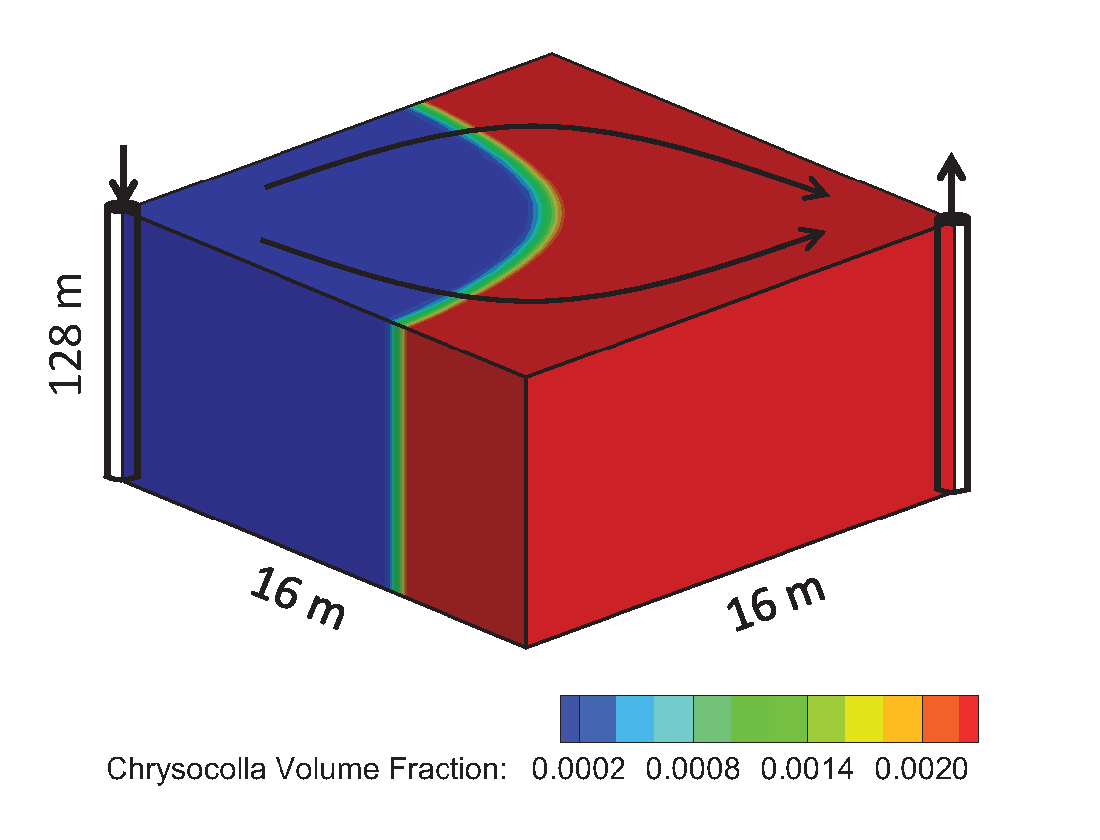
\includegraphics[width=0.95\linewidth]{./cu_leaching_schematic}
\end{center}
\end{frame}

%-----------------------------------------------------------------------------

\frame{
\frametitle{\bf Scaling: $32 \times 32 \times \magentacomment{4}$ Grid $\times 12$ Species}

\begin{itemize}
\item Scalabilty study performed on 1--1024 processor cores
\item Grid Resolution: $32 \times 32 \times \magentacomment{4}$
\item 49K degrees of freedom total (48 dof/core \@ 1024 cores)
\end{itemize}

\begin{center}
\includegraphics[width=2in]{./49K_runtime}
\includegraphics[width=2in]{./49K_runtime_zoom}
\end{center}
}

%-----------------------------------------------------------------------------
\frame{
\frametitle{\bf Speedup: $32 \times 32 \times \magentacomment{4}$ Grid $\times 12$ Species}
\begin{center}
\includegraphics[width=2in]{./49K_speedup}
\includegraphics[width=2in]{./49K_speedup_zoom}
\end{center}
}

%-----------------------------------------------------------------------------
\frame{
\frametitle{\bf Solver Iterations: $32 \times 32 \times \magentacomment{4}$ Grid $\times 12$ Species}
\begin{center}
\includegraphics[width=2in]{./49K_solver_iterations}
\end{center}
}

\end{document}
